\chapter{Proof of Concept}
\label{chap:proof-of-concept}
%\emph{This chapter presents and clarifies the results obtained during the research. The focus should be on the factual results, not the interpretation or discussion. Tables and graphics should be used to increase the clarity of the results where applicable.}
In Chapter~\ref{chap:research} we explained the difficulties of managing virtual networks and policies in \gls{dcos}. The main problem is that operators of clusters cannot get an overview of the created virtual networks and the applied network policies by \gls{cni} plugins. In this chapter we propose two solutions: first we explain how we could do this by expanding the \gls{cni} specification, next we report on the solution we implemented in the \gls{poc}. 

\section{Extending CNI}
\label{sec:expanding-cni}
One of the first ideas we had was to extend \gls{cni} to be bi-directional. This addition would allow operators to retrieve information about the virtual networks, to see which virtual networks are present and which containers are connected to the virtual network. The specification already has an \texttt{ADD} action that returns the network state of a container when it has been created. However this does not allow querying of the current state of the networks. It would require to create a custom solution to keep track of the current network state and follow the changes to the containers. To make this work we would have to adapt the \gls{cni} specification to include a new action to allow querying of the network state of containers. This new action could logically be called \texttt{GET}, returning the same information when the \texttt{ADD} action was invoked and allows for caching of the results.

We decided not to touch the CNI specification for this thesis, as it would have needed too much time: creating a new action in the \gls{cni} specification would require coordination and working together with different people and companies developing \gls{cni} plugins. At the beginning of this thesis the community was already discussing the need for a new action that would retrieve the current state of the network of a container. Maintainers did not agree yet on whether this should be implemented. Not only would we have to adjust the specification, we would also have to extend the \gls{cni} plugins in use at the client to support a new action. Furthermore this action will only expose information about the network state of the container, not the state of the virtual networks in the cluster which operators want to see. Network policies are not included in the \gls{cni} specification. With the new \texttt{GET} action in place we would still need a different solution for managing network policies. 

\section{Network Object API}
\label{sec:networkobject-api}
Instead of extending the \gls{cni} specification we decided to build a \gls{poc} for a new system in \gls{dcos}. A central \gls{api} in DC/OS for managing components related to virtual container network. We introduce a network object model. In this model an operator can define a network object with the relevant configuration for a network, very much like the objects used in the kube-apiserver. First we explain the model in Section~\ref{subsec:network-object-model}, next the global system design and features in Section~\ref{subsec:system-design} and we conclude with the implemented \gls{poc} in Section~\ref{subsec:poc-architecture}.

\subsection{Network Object Model}
\label{subsec:network-object-model}
The network object model contains different properties for defining networks in \gls{dcos}. The specification for this model can be found in Listing~\ref{lst:nom} and is written in Protocol buffers format. We explain the basic idea for each component. Note: this is a first version and can be evolved over time.

\lstinputlisting[label={lst:nom},caption={Network Object Model in Protocol buffers format},language=protobuf2,style=protobuf]{code/dcos_network_objects_v0.1.proto}

\begin{itemize}
    \item[\textbf{Virtual Network}] Specifies the basic properties of a network. Containing the name and subnet of a virtual network.
    \item[\textbf{Network Driver}] Driver for the specified network, which can be  a \gls{dcos} overlay network, a standard plugin, or a \gls{cni} plugin.
    \item[\textbf{Network Policy}] A set of firewall rules for a given network. These rules can be either level 4 rules for packet filtering based on port and host or level 7 rules to inspect on application level. Rules can also be applied based on labels to firewall specific applications or traffic.
    \item[\textbf{Network Service}] Services could be a set of different things to attach to a network. For example a cloud provider integration for ingress traffic to the cluster.
\end{itemize}

\subsection{Overall System Design}
\label{subsec:system-design}
The idea is that this new service runs on the masters of a \gls{dcos} cluster, residing in the networking box on the master nodes from Figure~\ref{fig:dcos-arch}. We choose the masters as they are already highly-available in a default setup. Both CockroachDB\cite{cockroachdb} and Zookeeper\cite{zookeeper} are already running on the master providing distributed storage for other \gls{dcos} components. It is also possible to use etcd\cite{etcd} as a central key-value store on the master. However this decision is out of scope for this thesis as the \gls{poc} in Section~\ref{subsec:poc-architecture} uses a different approach.

The system is based on the idea of the kube-apiserver from Kubernetes as discussed in Section~\ref{subsec:kubernetes} where an operator can query the current state and submit the required state. The system would not only provide insight to the available virtual networks and policies, but also be open to integrate with cloud providers for North-South traffic into the cluster for example. The new system should have the following features: 
\begin{itemize}
    \item Run highly available on the masters
    \item Use a distributed highly available storage solution
    \item Show an overview of the available virtual networks
    \item Allow to create, configure and delete virtual networks
    \item Give an overview of the applied network policies per network, tasks or framework
    \item Allow to create, configure and delete network policies
    \item Integrate with cloud providers to configure ingress traffic
\end{itemize}

\subsection{PoC Architecture}
\label{subsec:poc-architecture}
We want to show a basic \gls{poc} with a limited set of features where an operator can see and configure network policies for a given container on a virtual network. The code developed for this \gls{poc} can be accessed via an online repository hosted on Github\footnote{\url{https://github.com/wjglerum/dcos-networkobject-controller}\label{ftn:repo}}. Showing the available networks can be easily achieved with this new \gls{api} in place, however creating virtual networks is more difficult. To create a virtual network on demand we would have to distribute the plugin and its configuration to every node, configure and restart every agent in the cluster, which would require a custom build solution to achieve. Mesosphere is working on providing a system to distribute files to nodes for container volume mounts, which we could later use to distribute network specific files to every node.

Mesosphere recently added support for running Kubernetes on a \gls{dcos} cluster. We reuse the kube-apiserver with \glspl{crd} to submit and query network objects to be stored in etcd. A \gls{crd} is a custom object that works the same as other objects used by the kube-apiserver explained in Section~\ref{subsec:kubernetes}. This saves us from the burden of writing our own API server and setting it up manually on the masters. The kube-apiserver runs as a single container, however it depends on other Kubernetes components such as etcd to store information. Instead of trying to strip the kube-apiserver from Kubernetes components, we run an entire Kubernetes cluster on our \gls{dcos} cluster. This does cause some overhead, but we are still able to run a full cluster on a single Macbook Pro 2018 with 16GB of RAM. It did took some time to tune the CPU and memory usage to allow it to run on a single developer machine. For a production ready solution we should implement both the \gls{api} server and storage to run on the masters as discussed in Section~\ref{subsec:system-design}.

Next we created a custom controller written in GoLang\cite{golang} based on one of the examples provided by Kubernetes for dealing with \glspl{crd}. This controller listens to the updates on the kube-apiserver of a specific \gls{crd}. With a custom Dockerfile we can build a Docker container and run it on the \gls{dcos} cluster with Marathon. We connect it to the kube-apiserver allowing us to rapidly prototype and try out new queries for our network objects. The only difficulty is getting the configuration and credentials for access to the Kubernetes cluster in our custom controller. Luckily Marathon has support for volume mounts, so we can generate the configuration file once on the host allowing the container to read it from the volume mount to connect to the Kubernetes cluster.

\begin{figure}
    \centering
    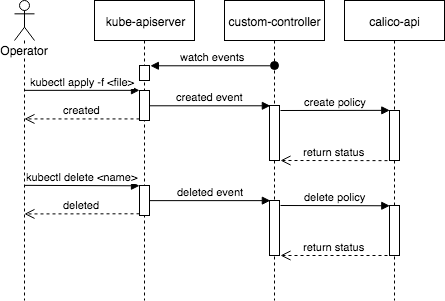
\includegraphics[width=0.75\columnwidth]{images/customer-controller-sequence-diagram}
    \caption{Sequence diagram for the custom controller}
    \label{fig:custrom-controller-sequence-diagram}
\end{figure}

When we submit a \gls{crd} containing a network object with network policies to the kube-apiserver, our custom controller listens for those events, see Figure~\ref{fig:custrom-controller-sequence-diagram}. Currently we support create, delete and list commands, updates are handled as a delete and create action to simplify the code base. In the case of an add command the controller checks which driver it is using, in our case only Project Calico is supported for now, and uses that plugin to create the network policies. In case of a delete command the controller removes the policy using the plugin. The state of the network policy is saved by the kube-apiserver in etcd and can be queried using the kubectl command from Kubernetes. Listing~\ref{lst:deploy} lists the step to to deploy all the components of this \gls{poc}, the addition JSON configuration files can be found online in the before mentioned repository. 
\lstinputlisting[label={lst:deploy},caption={Steps to deploy the PoC},language=bash]{code/deploy.sh}
Once the stack is up and running we can inspect the logs of the custom controller to see what is happening and interact with it using kubectl from our local machine. In short we use the following components for this \gls{poc}, visualised in Figure~\ref{fig:poc-stack}:
\begin{itemize}
    \item Local \gls{dcos} cluster running in VirtualBox\cite{virtualbox} using Vagrant\cite{vagrant},
    \item Kubernetes as a framework on \gls{dcos}, utilising the kube-apiserver with etcd to store our network objects,
    \item Custom controller listening for events and integrates with the Calico \gls{api}.
\end{itemize}


\begin{figure}
    \centering
    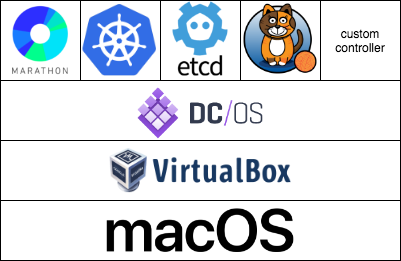
\includegraphics[width=0.6\columnwidth]{images/poc-stack}
    \caption{Technology stack of the proof of concept}
    \label{fig:poc-stack}
\end{figure}
